\chapter{Spin, Isospin, Farbe und Gluon-Selbstwechselwirkung}

\section{Quantenchromodynamik in Analogie zur Elektrodynamik}

Die Quantenchromodynamik ist ein zu großes Themengebiet, um es in einer einzigen Vorlesung vollständig zu behandeln. Hier geht es um das grundlegende anschauliche Bild, nicht um die tiefergehende Mathematik.

Die Quantenelektrodynamik ist die Theorie der Elektronen und Photonen. Sie ist auch die Quantentheorie der Coulomb-Kraft. Behandelt man den Atomkern als feste Quelle eines elektrischen Feldes und lässt seine Bewegung und innere Struktur außer Betracht, so ist die QED die Theorie des Atoms.

Die Quantenchromodynamik hat eine entsprechende Rolle für Quarks und Gluonen. Sie beschreibt die Teilchen selbst, die Kräfte zwischen ihnen und die zusammengesetzten Objekte, die sie bilden. Diese zusammengesetzten Teilchen heißen \emph{Hadronen}. Protonen und Neutronen sind Baryonen: Sie tragen eine von null verschiedene Gesamtquarkzahl oder, gleichbedeutend, eine von null verschiedene Baryonenzahl. Mesonen sind Quark--Antiquark-Kombinationen. Sowohl Baryonen als auch Mesonen enthalten außerdem Gluonen.

Gluonen sind elektrisch neutral, stellen aber das Feld bereit, das Quarks bindet. In dieser Hinsicht spielt das Gluonenfeld eine ähnliche Rolle wie das elektromagnetische Feld, das Atome bindet.

Bevor wir Farbe und Gluonen einführen, ist es hilfreich, zur Mathematik des Spins zurückzukehren. Dieselbe Mathematik tritt beinahe unmittelbar als \emph{Isospin} wieder auf; ein verwandtes Muster begegnet uns später erneut in der Theorie der Farbe. Diesen Konstruktionen liegt die Gruppentheorie zugrunde, doch die nötigen Ideen lassen sich anhand des Drehimpulses entwickeln.

\section{Drehimpulsmultipletts}

Die Drehimpulskomponenten erfüllen
\begin{equation}
[L_x,L_y]=i\hbar L_z,
\end{equation}
mit den zyklisch vertauschten Beziehungen
\begin{equation}
[L_y,L_z]=i\hbar L_x,
\qquad
[L_z,L_x]=i\hbar L_y.
\end{equation}
Die drei Komponenten kommutieren nicht miteinander und können daher nicht alle gleichzeitig gemessen werden. Eine Beschreibung wählt deshalb eine Achse aus, üblicherweise die \(z\)-Achse, und klassifiziert Zustände nach der Drehimpulskomponente entlang dieser Achse.

Diese Wahl bricht die Rotationssymmetrie der Natur nicht. Sie bricht die Symmetrie nur in der Beschreibung, indem sie für die Buchführung eine Richtung auswählt.

Die möglichen Werte der \(z\)-Komponente sind quantisiert und unterscheiden sich jeweils um eine Einheit \(\hbar\). Setzt man bei der Auflistung dieser Werte \(\hbar=1\), so enthält ein Multiplett mit Spin \(\ell\)
\begin{equation}
m=\ell,\ell-1,\ldots,-\ell.
\end{equation}
Die Zahl der unabhängigen Zustände beträgt somit
\begin{equation}
2\ell+1.
\end{equation}

Die ersten paar Multipletts seien ausdrücklich aufgeführt:
\begin{align}
\ell=0:&\qquad m=0,\\
\ell=\frac12:&\qquad m=\frac12,-\frac12,\\
\ell=1:&\qquad m=1,0,-1,\\
\ell=\frac32:&\qquad
m=\frac32,\frac12,-\frac12,-\frac32,\\
\ell=2:&\qquad m=2,1,0,-1,-2.
\end{align}

Für unsere Zwecke gilt: Halbzahliger Spin gehört zu Fermionen, ganzzahliger Spin zu Bosonen. Ein Elektron ist ein Teilchen mit Spin \(\tfrac12\). Ein Teilchen mit Spin null besitzt überhaupt keinen Drehimpuls. Das Photon hat Spin eins; Zustände mit Spin eins kommen auch bei Atomen und Kernen vor. Atome und Kerne können ebenso Spin \(\tfrac32\) haben, und die Zählung setzt sich für höhere Spins entsprechend fort.

Die Notation muss den Gesamtspin von seiner Komponente unterscheiden. Die Zahl \(\ell\) kennzeichnet das Multiplett und ist zugleich die größtmögliche \(z\)-Komponente. Die Zahl \(m\) kennzeichnet einen bestimmten Zustand innerhalb dieses Multipletts. Ein Objekt mit Spin eins hat also drei Zustände, ein Objekt mit Spin \(\tfrac12\) dagegen zwei.

\section{Kombination zweier Spin-Halb-Teilchen}

Betrachten wir zwei Teilchen mit Spin \(\tfrac12\) und vernachlässigen ihren Bahndrehimpuls. Ihr Spinproduktraum enthält vier Basiszustände:
\begin{equation}
|\uparrow\uparrow\rangle,\qquad
|\uparrow\downarrow\rangle,\qquad
|\downarrow\uparrow\rangle,\qquad
|\downarrow\downarrow\rangle.
\end{equation}
Die zugehörigen \(z\)-Komponenten sind
\begin{align}
|\uparrow\uparrow\rangle &: m=+1,\\
|\uparrow\downarrow\rangle &: m=0,\\
|\downarrow\uparrow\rangle &: m=0,\\
|\downarrow\downarrow\rangle &: m=-1.
\end{align}

Der Zustand, in dem beide Spins nach oben zeigen, belegt, dass ein Spin-eins-Multiplett vorkommen muss: Die maximale \(z\)-Komponente ist \(+1\). Ein Spin-eins-Multiplett hat nur drei Zustände,
\begin{equation}
m=+1,\quad 0,\quad -1.
\end{equation}
Der Produktraum enthält jedoch vier Zustände, darunter zwei unabhängige Zustände mit \(m=0\). Sie können nicht alle zu einem einzigen Spin-eins-Multiplett gehören. Der zusätzliche Zustand kann auch keinen Spin zwei haben, denn ein Spin-zwei-Multiplett müsste fünf Zustände enthalten. Die vier Produktzustände müssen sich folglich in drei Zustände mit Spin eins und einen Zustand mit Spin null aufteilen.

Welche Kombination der beiden \(m=0\)-Basiszustände gehört zum Spin-eins-Multiplett? Vertauschen wir die beiden Teilchen. Die gleichgerichteten Zustände bleiben unverändert:
\begin{equation}
|\uparrow\uparrow\rangle\longrightarrow|\uparrow\uparrow\rangle,
\qquad
|\downarrow\downarrow\rangle\longrightarrow|\downarrow\downarrow\rangle.
\end{equation}
Die gemischten Produktzustände werden dagegen vertauscht:
\begin{equation}
|\uparrow\downarrow\rangle
\longleftrightarrow
|\downarrow\uparrow\rangle.
\end{equation}
Ihre Summe ist unter der Vertauschung symmetrisch:
\begin{equation}
|\uparrow\downarrow\rangle+|\downarrow\uparrow\rangle.
\end{equation}
Die Normierung liefert den Faktor \(1/\sqrt2\):
\begin{equation}
|1,0\rangle
=
\frac{|\uparrow\downarrow\rangle
      +|\downarrow\uparrow\rangle}{\sqrt2}.
\end{equation}

\begin{figure}[h]
\centering
\includegraphics[width=0.78\textwidth]{lecture_02_figure_02.png}
\caption{Symmetrische Kombination der gemischten Spins, die das \(m=0\)-Mitglied des Spin-eins-Tripletts bildet.}
\lectureframe{00:15:08}
\end{figure}

Zusammen mit den beiden gleichgerichteten Zuständen ergibt sich so das Spin-eins-Triplett:
\begin{align}
|1,+1\rangle &=|\uparrow\uparrow\rangle,\\
|1,0\rangle &=
\frac{|\uparrow\downarrow\rangle
      +|\downarrow\uparrow\rangle}{\sqrt2},\\
|1,-1\rangle &=|\downarrow\downarrow\rangle.
\end{align}
Die verbleibende orthogonale Kombination enthält ein Minuszeichen:
\begin{equation}
|0,0\rangle
=
\frac{|\uparrow\downarrow\rangle
      -|\downarrow\uparrow\rangle}{\sqrt2}.
\end{equation}
Sie ist unter der Vertauschung antisymmetrisch und bildet das Ein-Zustands-Multiplett mit Spin null. Somit gilt:
\begin{equation}
\frac12\otimes\frac12=1\oplus0.
\end{equation}

Der symmetrische gemischte Spin-Zustand hat \(m=0\), aber er hat \emph{nicht} den Gesamtdrehimpuls null. Er gehört zum Spin-eins-Triplett. Bei einer Drehung der Koordinatenachsen mischt er sich mit den Zuständen \(m=\pm1\). Nur die antisymmetrische Kombination hat \(\ell=0\).

Was den Drehimpuls angeht, ist das Singulett wie leerer Raum. Es kann Energie, Ladung oder andere Quantenzahlen tragen, aber keinen Drehimpuls.

Diese Unterscheidung lässt sich mit einem Gedankenexperiment prüfen. Lassen wir alle Erhaltungssätze außer der Drehimpulserhaltung außer Acht und fragen, welcher Zweiteilchen-Spin-Zustand einfach verschwinden könnte. Keiner der beiden gleichgerichteten Zustände könnte verschwinden, da jeder zu einem Spin-eins-Multiplett gehört. Auch der symmetrische Zustand \(m=0\) könnte nicht verschwinden. Zwar verschwindet seine \(z\)-Komponente, sein Gesamtspin bleibt jedoch eins, mit nichttrivialen Komponenten bezüglich anderer Achsen. Nur das antisymmetrische Singulett könnte verschwinden, ohne die Drehimpulserhaltung zu verletzen.

\begin{classroomqa}
\audiencequestion{Würde eine Messung des symmetrischen gemischten Spin-Zustands entlang der \(z\)-Achse \(+1\) oder \(-1\) ergeben?\lecturetimestamp{00:19:28}}
\lecturerresponse{Nein. Entlang der \(z\)-Achse ergibt sie null. Der Zustand hat dennoch den Gesamtspin eins, sodass eine Messung entlang einer anderen Achse \(+1\) oder \(-1\) ergeben kann.}
\end{classroomqa}

\section{Drei Spin-Halb-Teilchen}

Kombinieren wir nun drei Teilchen mit Spin \(\tfrac12\). Es gibt
\begin{equation}
2\times2\times2=8
\end{equation}
Produktzustände. Zeigen alle drei Spins nach oben, so beträgt die gesamte \(z\)-Komponente \(+\tfrac32\). Daher muss ein Multiplett mit Spin \(\tfrac32\) vorkommen. Es enthält
\begin{equation}
2\left(\frac32\right)+1=4
\end{equation}
Zustände.

Vier Zustände bleiben übrig. Sie können kein zweites Multiplett mit Spin \(\tfrac32\) bilden, denn die Zustände mit \(m=\pm\tfrac32\) sind bereits verwendet. Die verbleibenden Zustände haben als maximale Komponenten nur \(+\tfrac12\) und \(-\tfrac12\). Drei halbzahlige Spins können auch keinen Gesamtspin null ergeben. Die übrigen Zustände müssen Multipletts mit Spin \(\tfrac12\) bilden.

Ein Multiplett mit Spin \(\tfrac12\) enthält zwei Zustände. Da vier Zustände übrig sind, gibt es zwei verschiedene Multipletts mit Spin \(\tfrac12\):
\begin{equation}
\frac12\otimes\frac12\otimes\frac12
=
\frac32\oplus\frac12\oplus\frac12.
\end{equation}
Dieses Muster wird wiederkehren, wenn die beiden Zustände namens Spin-up und Spin-down durch die beiden Quarkflavours up und down ersetzt werden.

\section{Isospin als innerer Spin}

Isospin, auch isotopischer Spin genannt, ist ein inneres Analogon des gewöhnlichen Spins. Der gewöhnliche Spin ist an Drehungen des physikalischen Raums gebunden, der Isospin nicht. Er betrifft Transformationen in einem inneren mathematischen Raum, dessen zwei Grundzustände wir identifizieren mit
\begin{equation}
u,\qquad d.
\end{equation}
Die Bezeichnungen \emph{up} und \emph{down} dienen hier lediglich als Flavour-Bezeichnungen. Im gewöhnlichen Raum zeigt nichts nach oben oder unten.

\editorialnote{Ein kurzer Übergang zwischen der Definition des inneren Spinraums und dem folgenden Argument zur hadronischen Massenskala lässt sich nicht zuverlässig rekonstruieren. Daraus wird keine zusätzliche physikalische Aussage abgeleitet.}

Warum eignen sich \(u\) und \(d\) für diese Analogie? Die natürliche Energieskala der Hadronenphysik liegt bei einigen hundert MeV. Ein typisches leichtes Meson hat eine Masse von einigen hundert MeV, und auch die Energie, die beim Binden dreier Quarks zu einem Nukleon beteiligt ist, liegt in dieser Größenordnung. Im Vergleich dazu betragen die Bindungsenergien gewöhnlicher Atomkerne nur einige MeV. Die Kraft, die Protonen und Neutronen innerhalb eines Kerns zusammenhält, wird somit auf einer viel kleineren Energieskala betrachtet als die Dynamik, die Quarks innerhalb eines Hadronen bindet.

Von den sechs Quarkflavours sind \(u\) und \(d\) im Vergleich zur hadronischen Skala leicht. Schwere Quarks erfordern mehr Energie zu ihrer Erzeugung, und Hadronen, die sie enthalten, können in leichtere zerfallen. Die stabilsten leichten Hadronen bestehen daher aus up- und down-Quarks.

Das down-Quark ist schwerer als das up-Quark, nach den hier verwendeten Schätzungen ungefähr um den Faktor zwei; beide Massen sind jedoch klein im Vergleich zu einigen hundert MeV. In erster Näherung können beide auf der hadronischen Skala als nahezu masselos behandelt werden. Noch wichtiger ist, dass man ihre Massen als nahezu gleich ansetzen kann.

Diese ungefähre Gleichheit führt zu einer Symmetrie. Werden up- und down-Quarks vertauscht, ändert sich die Physik der starken Wechselwirkung nur sehr wenig. Das Proton,
\begin{equation}
p\sim uud,
\end{equation}
und das Neutron,
\begin{equation}
n\sim udd,
\end{equation}
sind das einfachste Beispiel: Sie unterscheiden sich durch die Vertauschung von \(u\) und \(d\), und ihre Massen sind sehr ähnlich.

Die Vertauschung
\begin{equation}
u\longleftrightarrow d
\end{equation}
wird daher mathematisch wie
\begin{equation}
|\uparrow\rangle\longleftrightarrow|\downarrow\rangle.
\end{equation}
behandelt. Beim gewöhnlichen Spin entspricht die Transformation einer Drehung einer Achse im Raum. Beim Isospin ist sie eine Drehung in einem inneren Raum. Die Mathematik ist analog, obwohl die physikalischen Bedeutungen verschieden sind.

\begin{figure}[h]
\centering
\includegraphics[width=0.80\textwidth]{lecture_02_figure_03.png}
\caption{Zerlegung in Triplett und Singulett für zwei Zustände mit Spin \(\tfrac12\), als Modell für die entsprechende Isospin-Konstruktion.}
\lectureframe{00:27:42}
\end{figure}

Das Präfix \emph{iso} stammt von \emph{Isotop}. In der älteren Beschreibung des Atomkerns galten Proton und Neutron als zwei Mitglieder eines inneren Dubletts. Werden in einem Kern Proton und Neutron vertauscht, entsteht ein anderes Isotop. Das Quarkmodell führte diese Vertauschung von Proton und Neutron später auf die zugrunde liegende Vertauschung von \(u\) und \(d\) zurück.

\begin{classroomqa}
\audiencequestion{Gab es den Isospin schon vor dem Quarkmodell?\lecturetimestamp{00:30:19}}
\lecturerresponse{Ja. Der Isospin wurde vor der Einführung der Quarks eingeführt und ist historisch mit Heisenberg verbunden. Das Quarkmodell lieferte später seine Deutung in Form der \(u\)- und \(d\)-Flavours.}
\end{classroomqa}

Der Isospin ist keine exakte Symmetrie der Natur. Die Massen der up- und down-Quarks sind nicht genau gleich, und ihre elektrischen Ladungen unterscheiden sich:
\begin{equation}
Q(u)=+\frac23,
\qquad
Q(d)=-\frac13.
\end{equation}
Selbst bei gleichen Massen würde der Elektromagnetismus sie weiterhin unterscheiden.

In kleinen hadronischen und nuklearen Systemen sind elektromagnetische Effekte im Vergleich zur starken Wechselwirkung schwach. In einem großen Atomkern kann die elektrische Abstoßung wichtig werden; bei einem Proton, einem Neutron oder einem kleinen Kern wie Helium ist sie eine vergleichsweise kleine Korrektur auf der Skala der starken Wechselwirkung. Die Isospin-Näherung umfasst daher zwei Schritte:

\begin{enumerate}
\item den Massenunterschied zwischen \(u\)--\(d\) vernachlässigen;
\item ihre elektromagnetische Unterscheidung ausschalten und nur die starke Wechselwirkung berücksichtigen.
\end{enumerate}

In dieser Näherung wird die Transformation zwischen \(u\) und \(d\) zu einer mathematischen Symmetrie, die der Symmetrie des gewöhnlichen Spins analog ist.

\section{Das Nukleon-Isospin-Dublett}

Ein einzelnes Quark lässt sich nicht isolieren und als freies Objekt im Labor untersuchen. Die einfachsten beobachteten Baryonen enthalten drei Quarks. Das Zählargument für drei Spins hat daher ein direktes Isospin-Analogon: Drei Quarks mit Isospin \(\tfrac12\) können einen Gesamtisospin \(\tfrac32\) oder \(\tfrac12\) bilden.

Beginnen wir mit dem Gesamtisospin \(\tfrac12\). Ein solches Multiplett hat
\begin{equation}
2\left(\frac12\right)+1=2
\end{equation}
Zustände. Sie sind das Proton und das Neutron:
\begin{equation}
p\sim uud,
\qquad
n\sim udd.
\end{equation}
Ihre Ladungen sind
\begin{align}
Q(p)
&=\frac23+\frac23-\frac13
=+1,\\
Q(n)
&=\frac23-\frac13-\frac13
=0.
\end{align}
Die Vertauschung von \(u\) und \(d\) vertauscht Proton und Neutron. Sie bilden ein Isospin-\(\tfrac12\)-Dublett.

Um die Austausch-Symmetrie zu besprechen, versehen wir drei Quarkplätze vorübergehend mit den Bezeichnungen \(1,2,3\). Diese Bezeichnungen sind nicht als feste Quarkpositionen zu verstehen; die Quarks bewegen sich. Ein schematischer Protonfaktor lautet
\begin{equation}
d_1\bigl(u_2u_3-u_3u_2\bigr).
\end{equation}

\begin{figure}[h]
\centering
\includegraphics[width=0.58\textwidth]{lecture_02_figure_04.png}
\caption{Antisymmetrisierter Zwei-\(u\)-Quark-Faktor in einem schematischen Protonzustand.}
\lectureframe{00:35:43}
\end{figure}

Der Ausdruck soll die Antisymmetrie beim Austausch von Fermionen hervorheben. Er ist keine vollständige Proton-Wellenfunktion. Der vollständige Zustand muss Flavour, gewöhnlichen Spin, räumliche Abhängigkeit und---wie gleich deutlich wird, unverzichtbar--- Farbe kombinieren.

\editorialnote{Die Indizes sind vorübergehende Platz- oder Einteilchenbezeichnungen. Zwei identische \(u\)-Flavourzustände bilden nicht das übliche antisymmetrische Isospin-Singulett; der dargestellte Faktor allein erlaubt daher keinen Schluss auf Isospin null. Er wird hier nur als lokaler Schritt zur Antisymmetrisierung der Plätze beibehalten; der Gesamtisospin des Protons folgt aus seinem vollständigen Drei-Quark-Zustand.}

Der begrenzte Vergleich mit der vorherigen Spin-Konstruktion besteht darin, dass sich Quantenzustände bezüglich eines Austauschs von Bezeichnungen symmetrisch oder antisymmetrisch kombinieren lassen. Dieser Vergleich allein bestimmt nicht den Isospin des dargestellten \(uu\)-Faktors.

Das Proton hat sowohl den gewöhnlichen Spin \(\tfrac12\) als auch den Isospin \(\tfrac12\). Für das Neutron gilt dasselbe. Dies sind verschiedene Quantenzahlen: Der gewöhnliche Spin betrifft physikalische Drehungen, der Isospin dagegen die innere \(u\)--\(d\)-Symmetrie.

\section{Das Delta-Quartett}

Drei leichte Quarks können auch einen Gesamtisospin \(\tfrac32\) bilden. Das resultierende Multiplett aus vier Zuständen ist das Delta-Quartett:
\begin{equation}
\begin{aligned}
\Delta^{++}&\sim uuu,
&
\Delta^{+}&\sim uud,
\\
\Delta^{0}&\sim udd,
&
\Delta^{-}&\sim ddd.
\end{aligned}
\end{equation}
Die Delta-Zustände haben neben dem Isospin \(\tfrac32\) auch den gewöhnlichen Spin \(\tfrac32\). In den Zuständen mit maximalen Komponenten sind die drei gewöhnlichen Spins gleichgerichtet, ebenso die drei Isospins.

Eine Zusammensetzung wie \(uud\) bestimmt für sich genommen nicht, ob der Zustand ein Proton oder ein \(\Delta^+\) ist. Derselbe Flavourinhalt lässt sich zu Zuständen mit unterschiedlichem Gesamtspin und Gesamtisospin kombinieren.

\begin{classroomqa}
\audiencequestion{Was unterscheidet das \(uud\)-Mitglied des Delta-Quartetts von einem Proton?\lecturetimestamp{00:41:08}}
\lecturerresponse{Ihre gewöhnlichen Spins unterscheiden sich. Das Proton hat Spin \(\tfrac12\), während der Delta-Zustand Spin \(\tfrac32\) hat. Die Quarks sind außerdem zu Zuständen mit verschiedenem Gesamtisospin kombiniert.}
\end{classroomqa}

\begin{classroomqa}
\audiencequestion{Sind die beiden mittleren Mitglieder des Delta-Quartetts Isospin-\(\tfrac12\)-Zustände?\lecturetimestamp{00:41:52}}
\lecturerresponse{Nein. Ihre Isospin-Komponenten sind \(+\tfrac12\) und \(-\tfrac12\), ihr Gesamtisospin ist jedoch \(\tfrac32\). Ein Multiplett mit Gesamtisospin \(\tfrac32\) enthält notwendigerweise vier Komponenten-Zustände.}
\end{classroomqa}

Die vier Isospin-Komponenten entsprechen
\begin{equation}
I_3=\frac32,\frac12,-\frac12,-\frac32.
\end{equation}
Ihre elektrischen Ladungen sind
\begin{align}
Q(\Delta^{++})&=+2,\\
Q(\Delta^{+})&=+1,\\
Q(\Delta^{0})&=0,\\
Q(\Delta^{-})&=-1.
\end{align}
Die Ladungen der beiden mittleren Zustände entsprechen zufällig den Ladungen von Proton und Neutron; die Zustände bleiben jedoch verschieden, weil ihre Spin- und Isospin-Kopplungen unterschiedlich sind.

Aufgrund der näherungsweisen Isospin-Symmetrie sind die vier Delta-Massen nahezu gleich. Der kleine Massenunterschied zwischen \(u\)--\(d\) bewirkt nur eine geringe Aufspaltung des Quartetts. Die gemeinsame Massenskala der Deltas beträgt ungefähr
\begin{equation}
m_\Delta\sim1200\,\mathrm{MeV},
\end{equation}
während Proton und Neutron nahe bei
\begin{equation}
m_N\sim940\,\mathrm{MeV}.
\end{equation}liegen.

\subsection{Zerfall des \texorpdfstring{\(\Delta^{++}\)}{Delta++}}

Die Delta-Zustände sind schwer genug, um in ein Nukleon und ein Pion zu zerfallen. Betrachten wir
\begin{equation}
\Delta^{++}\sim uuu.
\end{equation}
Wenn sich die Bestandteile voneinander entfernen, kann ein Quark--Antiquark-Paar erzeugt werden. Eine versuchte Einfügung eines \(u\bar u\) würde im Endzustand ein Baryon aus drei \(u\) hinterlassen und bei der verfügbaren Energie keinen leichteren erlaubten Zerfallskanal eröffnen. Stattdessen erlaubt die Erzeugung eines \(d\bar d\)-Paars, dass sich die Bestandteile neu gruppieren zu
\begin{equation}
uuu+d\bar d
\longrightarrow
uud+u\bar d.
\end{equation}
Die beiden zusammengesetzten Endzustände sind
\begin{equation}
uud=p,
\qquad
u\bar d=\pi^+,
\end{equation}
also gilt
\begin{equation}
\Delta^{++}\longrightarrow p+\pi^+.
\end{equation}

\begin{figure}[h]
\centering
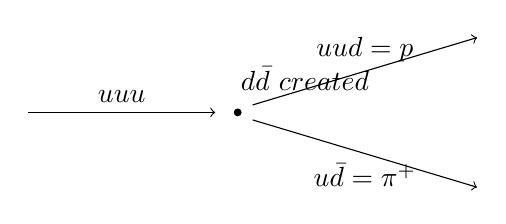
\begin{tikzpicture}[scale=0.95]
\draw[->] (-3,0) -- (-0.5,0) node[midway,above] {$uuu$};
\fill (-0.2,0) circle (1.5pt);
\draw[->] (0,0.1) -- (3,1.0) node[midway,above] {$uud=p$};
\draw[->] (0,-0.1) -- (3,-1.0) node[midway,below] {$u\bar d=\pi^+$};
\node at (0.7,0.45) {$d\bar d\ \text{created}$};
\end{tikzpicture}
\caption{Neugruppierung der Bestandteile beim Zerfall \(\Delta^{++}\rightarrow p+\pi^+\).}
\end{figure}

Die Ladungserhaltung ist unmittelbar ersichtlich:
\begin{equation}
Q(p)+Q(\pi^+)=1+1=2=Q(\Delta^{++}).
\end{equation}
Auch die grobe Massenbilanz lässt den Zerfall zu:
\begin{equation}
1200\,\mathrm{MeV}
>
940\,\mathrm{MeV}+140\,\mathrm{MeV}.
\end{equation}
Es bleibt genügend Energie für kinetische Energie im Endzustand.

Alle vier Delta-Zustände können in ein Proton oder Neutron zusammen mit einem Pion zerfallen. Ihre Lebensdauern sind extrem kurz. Eine Abschätzung der Größenordnung ergibt sich aus der Zeit, die Licht braucht, um ein Proton zu durchqueren:
\begin{equation}
\tau_\Delta
\sim
\frac{10^{-13}\,\mathrm{cm}}
     {10^{10}\,\mathrm{cm/s}}
\sim10^{-23}\,\mathrm{s}.
\end{equation}
Sie leben dennoch lange genug, um als unterschiedliche Objekte identifiziert zu werden, die bei Teilchenkollisionen entstehen.

\begin{classroomqa}
\audiencequestion{Ist bei dieser Buchführung der Bestandteile die geschriebene Reihenfolge der Symbole \(u\) und \(d\) von Bedeutung?\lecturetimestamp{00:48:49}}
\lecturerresponse{Für den vorliegenden Zweck nicht. Entscheidend sind der Flavourinhalt und die Art, wie der vollständige Quantenzustand zusammengesetzt ist.}
\end{classroomqa}

\section{Das Pauli-Rätsel und die Notwendigkeit der Farbe}

Das \(\Delta^{++}\) führt zu einem Widerspruch. Es besteht aus drei up-Quarks. In einem Zustand mit Spin \(\tfrac32\) können ihre gewöhnlichen Spins alle in dieselbe Richtung zeigen. Auch ihre Isospins sind identisch, denn sie sind alle \(u\). Wären Spin, Flavour und der räumliche Zustand niedrigster Energie die vollständige Beschreibung, so wären die drei Quarks identische Fermionen im selben Zustand. Das Pauli-Ausschlussprinzip verbietet dies.

\begin{classroomqa}
\audiencequestion{Wie können die wiederholt auftretenden up-Quarks Fermionen sein, wenn sie anscheinend denselben Zustand besetzen?\lecturetimestamp{00:48:58}}
\lecturerresponse{Sie können nicht in sämtlichen Quantenzahlen identisch sein. Das \(\Delta^{++}\) zeigt, dass Quarks neben gewöhnlichem Spin, Flavour und räumlichem Zustand eine zusätzliche Bezeichnung benötigen. Diese zusätzliche Bezeichnung ist die Farbe.}
\end{classroomqa}

Die neue Bezeichnung kann drei Werte annehmen:
\begin{equation}
r,\qquad g,\qquad b,
\end{equation}
genannt rot, grün und blau. Diese Wörter haben nichts mit sichtbaren Farben zu tun. Es sind beliebige Namen für drei innere Zustände. Man hätte auch andere Namen verwenden können; entscheidend ist, dass es drei verschiedene Möglichkeiten gibt.

Die roten, grünen und blauen Varianten eines bestimmten Quark-Flavours haben dieselbe Masse und dieselben gewöhnlichen beobachtbaren Eigenschaften. Dennoch sind sie verschiedene Quantenzustände. Ein \(\Delta^{++}\) kann daher ein rotes \(u\), ein grünes \(u\) und ein blaues \(u\) enthalten, sodass die drei Fermionen nicht denselben vollständigen Zustand besetzen.

Die sechs Flavours sind
\begin{equation}
u,\ d,\ c,\ s,\ t,\ b.
\end{equation}
Diese Reihenfolge richtet sich nicht nach der Masse. Das up-Quark ist das leichteste, darauf folgt das down-Quark. Das charm-Quark ist wesentlich schwerer als das strange-Quark, und das top-Quark ist sehr viel schwerer als das bottom-Quark. Jedes Flavour kommt in drei Farben vor. Ein Quark trägt daher mindestens zwei verschiedene innere Bezeichnungen:
\begin{equation}
\text{flavor}\quad\text{and}\quad\text{color}.
\end{equation}

Könnten die drei Quarks stattdessen durch Position oder Impuls unterschieden werden? Das Delta-Rätsel betrifft den Zustand niedrigster Energie, in dem die relevante räumliche Struktur und Impulsstruktur keine drei verschiedenen Bezeichnungen liefern können, ohne die Energie- und Symmetrieeigenschaften zu verändern. Die fehlende Unterscheidung muss eine neue innere Freiheitsgrad sein.

Eine aufschlussreiche Analogie bietet die Rolle des Spins in der Atomphysik. Zwei Elektronen, die scheinbar denselben Orbitalzustand besetzen, können sich dennoch durch ihren Spin-Zustand unterscheiden. Auf dieselbe strukturelle Weise können sich Quarks, die in Flavour, gewöhnlichem Spin und räumlichem Zustand übereinstimmen, durch ihre Farbe unterscheiden.

\editorialnote{Der genaue historische Ablauf im Zusammenhang mit Helium-Spektroskopie, dem Pauli-Prinzip sowie Uhlenbeck und Goudsmit wurde ausdrücklich als unsicher eingestuft. Die Analogie bleibt erhalten, ohne zu behaupten, dass dies der genaue zeitliche Ablauf der Entdeckung des Spins war.}

Yoichiro Nambu wird mit der Erkenntnis in Verbindung gebracht, dass Quarks diesen zusätzlichen Freiheitsgrad benötigen. Die physikalische Aussage hängt nicht von seiner Bezeichnung ab: Drei Quarkfarben lösen den Widerspruch mit dem Pauli-Prinzip. Das maßgebliche Ausschlussprinzip ist das Pauli-Prinzip, nicht die Heisenbergsche Unschärferelation.

\editorialnote{Die genaue Zuschreibung und spätere Geschichte der Bezeichnung \emph{Farbe} blieb unklar; daher wird hier kein genauerer zeitlicher Ablauf behauptet. Eine mündliche Bezugnahme auf die Heisenbergsche Unschärferelation wird entsprechend dem Zusammenhang mit der Fermionenstatistik zum Pauli-Ausschlussprinzip berichtigt.}

Dieselbe Farbkonstruktion gilt für Proton und Neutron. Ihre Zustände entstehen nicht dadurch, dass jeder geschriebenen Flavour-Bezeichnung dauerhaft eine bestimmte Farbe zugewiesen wird. Ein physikalisches Baryon ist eine quantenmechanische Superposition der möglichen Zuordnungen von Rot, Grün und Blau, kombiniert mit den geeigneten Austauschsymmetrien.

\begin{classroomqa}
\audiencequestion{Ist Farbe eine gewöhnliche physikalische Eigenschaft, die sich direkt messen lässt?\lecturetimestamp{00:56:55}}
\lecturerresponse{Die drei Farben haben dieselbe Masse und dieselben gewöhnlichen Eigenschaften. Ihre Unterscheidung zeigt sich in Beziehungen, nämlich durch erlaubte Kombinationen und Kollisionsprozesse. Experimente belegen, dass es drei verschiedene Farbzustände gibt, obwohl sich kein isoliertes farbiges Quark zur direkten Untersuchung präparieren lässt.}
\end{classroomqa}

\begin{classroomqa}
\audiencequestion{Ist Farbe erhalten?\lecturetimestamp{00:57:38}}
\lecturerresponse{Ja. Farbe ist erhalten, aber die hier betrachteten beobachtbaren Teilchen haben stets Farbe null, weshalb dies ein etwas ungewöhnlich wirkendes Erhaltungsgesetz ist.}
\end{classroomqa}

\editorialnote{Genauer gesagt sind asymptotische Hadronen Farbsinguletts. Die Formulierung ``Farbe null'' bezeichnet keine abelsche Nettoladung, die sich durch numerisches Addieren von Rot, Grün und Blau ergibt.}

\begin{classroomqa}
\audiencequestion{Benötigt das \(uud\)Proton für sich genommen wirklich alle drei Farben? Es scheint doch zu genügen, die beiden \(u\)-Quarks voneinander zu unterscheiden.\lecturetimestamp{00:57:58}}
\lecturerresponse{Dieses Beispiel zeigt zwar unmittelbar, dass irgendeine zusätzliche Unterscheidung nötig ist, macht die Zahl drei aber nicht zwingend. Das \(\Delta^{++}\) mit drei up-Quarks, deren gewöhnliche Spins und Isospins parallel sind, belegt eindeutig, dass drei verschiedene Bezeichnungen nötig sind.}
\end{classroomqa}

Deshalb spielte das Delta eine so wichtige Rolle. Proton und Neutron haben kompliziertere Spin- und Flavour-Symmetrien, sodass der Widerspruch durch die Einzelheiten ihrer Wellenfunktionen verdeckt werden kann. Beim \(\Delta^{++}\) ist der Konflikt unmittelbar:
\begin{equation}
uuu,\qquad
\uparrow\uparrow\uparrow,
\qquad
\text{one lowest spatial state}.
\end{equation}
Eine neue Bezeichnung mit drei möglichen Werten ist erforderlich. Die Existenz von drei Farbzuständen wird außerdem unabhängig durch Daten aus Hadronenkollisionen bestätigt.

Eine Symmetriebezeichnung kann bedeutsam sein, auch wenn ihre Alternativen für sich genommen gleichwertig sind. Ohne eine ausgewählte räumliche Achse sind zwei Spinrichtungen physikalisch gleichwertig. Ein zweites Objekt kann eine Bezugsachse bereitstellen und ihre Beziehung sichtbar machen. Ebenso legt ein Proton oder Neutron eine Richtung im Isospinraum fest; Vergleiche mit anderen Zuständen zeigen, ob innere Ausrichtungen parallel oder antiparallel sind. Farbe ist subtiler, aber auch ihr physikalischer Gehalt zeigt sich durch Beziehungen, Korrelationen und Wechselwirkungsregeln, nicht durch sichtbare Färbung.

Man könnte stattdessen erwägen, das Pauli-Prinzip aufzugeben. Dafür wäre ein neues mathematisches Rahmenwerk nötig: Die gewöhnliche Quantenfeldtheorie klassifiziert Teilchen als Fermionen oder Bosonen und bietet keine etablierte dritte Möglichkeit, die dieses Problem löst. Die QCD behält den fermionischen Charakter der Quarks bei und führt Farbe ein.

\begin{classroomqa}
\audiencequestion{Welche beobachtbare Größe entspricht der verborgenen Unterscheidung, die das Pauli-Prinzip erfordert?\lecturetimestamp{01:01:08}}
\lecturerresponse{Diese Frage ist wesentlich subtiler als die vertrauten Observablen Position, Impuls oder Isospin. Für eine vollständige Antwort sind weitere Aspekte der Farbdynamik erforderlich; sie wird deshalb auf später verschoben.}
\end{classroomqa}

\begin{classroomqa}
\audiencequestion{Wurde auf den fermionischen Charakter der Quarks anhand der Spin-Zuordnungen der Hadronen geschlossen?\lecturetimestamp{01:01:43}}
\lecturerresponse{Ja.}
\end{classroomqa}

\editorialnote{Der Wortlaut der beiden vorangegangenen Fragen aus dem Publikum ist teilweise undeutlich. Ihre Themen und die knappen Antworten sind gesichert; eine ausführlichere Formulierung wird nicht abgeleitet.}

\begin{classroomqa}
\audiencequestion{Wie kann man einem bestimmten Quark in einem Proton eine bestimmte Farbe zuordnen?\lecturetimestamp{01:01:55}}
\lecturerresponse{Man ordnet keinem dauerhaft identifizierbaren Bestandteil eine feste Farbe zu. Das Proton ist eine quantenmechanische Superposition aller erlaubten Zuordnungen von Rot, Grün und Blau; die Spin-, Flavour-, Raum- und Farbfaktoren werden dabei entsprechend symmetrisiert oder antisymmetrisiert. Das \(\Delta^{++}\) ist hilfreich, weil seine parallele Spin- und Flavour-Struktur den Bedarf an Farbe offenlegt, ohne dass man die vollständige Proton-Wellenfunktion benötigt.}
\end{classroomqa}

Farbe verhält sich zur QCD wie die elektrische Ladung zur Elektrodynamik: Sie ist die Quantenzahl, welche die Wechselwirkung steuert. Die QCD beschreibt experimentelle Daten aus Hadronenkollisionen mit hoher Genauigkeit. Letztlich ist der Rahmen dadurch gerechtfertigt, dass seine Konsequenzen mit dem Experiment übereinstimmen.

\section{Photonen und Gluonen}

Quarks sind die fermionischen Materieteilchen der QCD und ähneln in dieser Hinsicht den Elektronen in der QED. Was bindet sie?

In der Elektrodynamik ist ein Elektron eine Quelle des elektromagnetischen Feldes. In der Sprache der Teilchen emittiert und absorbiert es Photonen; der Austausch von Photonen erzeugt Kräfte zwischen geladenen Teilchen. Entsprechend ist ein Quark eine Quelle des Gluonenfeldes und kann Gluonen emittieren und absorbieren.

Gluonen ähneln Photonen in mehreren wichtigen Eigenschaften. Sie sind masselose Teilchen mit Spin eins und haben photonähnliche Polarisationszustände. Impuls und Polarisation sind gewöhnliche dynamische Eigenschaften. Der entscheidende Unterschied besteht darin, dass Gluonen Farbinformation tragen und deshalb miteinander wechselwirken.

Photonen tragen keine elektrische Ladung. Auf der elementaren Ebene der QED emittiert ein Photon kein weiteres Photon, und zwei Lichtstrahlen durchdringen einander, ohne miteinander zu wechselwirken. Es gibt sehr kleine Photon-Photon-Wechselwirkungen höherer Ordnung, an denen Elektronenschleifen beteiligt sind; diese sind jedoch sekundäre Effekte und keine direkte Photon-Selbstkopplung. Im leeren Raum besteht der elementare QED-Vertex einfach darin, dass ein Elektron ein Photon emittiert oder absorbiert.

\begin{figure}[h]
\centering
\begin{tikzpicture}[scale=1.0]
\draw[->] (-2,-1) -- (0,0);
\draw[->] (0,0) -- (2,-1);
\draw[smooth] plot coordinates {
(0,0) (0.16,0.27) (0.32,0.23) (0.48,0.52)
(0.64,0.48) (0.80,0.77) (0.96,0.73)
(1.12,1.02) (1.28,0.98) (1.44,1.27)
(1.60,1.23) (1.76,1.52)
};
\node at (-1.25,-0.75) {$e^-$};
\node at (1.25,-0.75) {$e^-$};
\node at (1.95,1.62) {$\gamma$};
\fill (0,0) circle (1.5pt);
\end{tikzpicture}
\caption{Elementarer QED-Vertex: Ein Elektron emittiert oder absorbiert ein Photon.}
\end{figure}

Wird die Richtung einer Fermionlinie umgekehrt, geht die Interpretation des Elektrons in die eines Positrons über. Emission, Absorption und gekreuzte Positronprozesse sind allesamt Umdeutungen dieses einen Vertex.

Zur Buchführung kann man sich vorstellen, ein Photon habe einige Eigenschaften eines Elektron--Positron-Paares. Das Paar ist elektrisch neutral, und ausgerichtete Elektron- und Positronspins können zusammen den Gesamtspin eins ergeben. Wenn eine äußere Wechselwirkung die erforderliche Energie und den erforderlichen Impuls bereitstellt, kann ein Photon ein Elektron--Positron-Paar erzeugen. Das bedeutet keineswegs, dass ein Photon buchstäblich aus einem Elektron und einem Positron besteht. Das Bild eines fiktiven Paares trägt wenig zum Verständnis der QED selbst bei, doch seine Farbanalogie ist in der QCD nützlich.

\section{Farbe--Antifarbe-Bezeichnungen für Gluonen}

Man stelle die drei Farbzustände eines Quarks als Spaltenvektor dar:
\begin{equation}
q=
\begin{pmatrix}
r\\
g\\
b
\end{pmatrix}.
\end{equation}
Die entsprechenden Antiquark-Bezeichnungen stelle man als Zeilenvektor dar:
\begin{equation}
\bar q=
\begin{pmatrix}
\bar r&\bar g&\bar b
\end{pmatrix}.
\end{equation}

Ein Gluon ist kein gebundener Zustand aus Quark--und Antiquark. Dennoch verhält sich seine Farbbuchführung so, als trüge es eine Farbe und eine Antifarbe. Die möglichen Bezeichnungen lassen sich daher wie folgt anordnen:
\begin{equation}
\begin{pmatrix}
r\bar r&r\bar g&r\bar b\\
g\bar r&g\bar g&g\bar b\\
b\bar r&b\bar g&b\bar b
\end{pmatrix}.
\end{equation}
Auf den ersten Blick ergeben sich so neun Kombinationen.

\begin{classroomqa}
\audiencequestion{Sind die Diagonaleinträge mit Farbe--und Antifarbe nicht unterscheidbar?\lecturetimestamp{01:13:37}}
\lecturerresponse{Nicht einfach so. Die Diagonaleinträge sind verschieden; entscheidend ist, dass ihre Summe keinen unabhängigen Quantenzustand bildet.}
\end{classroomqa}

Tatsächlich gibt es nur acht unabhängige Gluonzustände. Die drei Diagonalbezeichnungen sind nicht einfach untereinander ununterscheidbar, aber die spezielle Diagonalsumme
\begin{equation}
r\bar r+g\bar g+b\bar b
\end{equation}
ist kein zusätzliches unabhängiges Gluon der QCD. Die genauere Erklärung dieser Reduktion folgt später. Für die vorliegenden Argumente zum Farbfluss ist es nützlich, mit den neun scheinbaren Bezeichnungen zu arbeiten und sich zu merken, dass eine Diagonalkombination fehlt.

\section{Der Quark--Gluon-Vertex}

Ein Quark kann ein Gluon emittieren und dabei dieselbe oder eine andere Farbe annehmen. Tritt ein Quark mit der Farbe \(a\)ein und verlässt es den Vertex mit der Farbe \(b\), trägt das emittierte Gluon die Buchführungsbezeichnung \(a\bar b\):
\begin{equation}
a\longrightarrow b+(a\bar b).
\end{equation}
Zum Beispiel:
\begin{equation}
r\longrightarrow g+(r\bar g).
\end{equation}
Die rote Farblinie setzt sich im Gluon fort, während die grüne Linie durch das auslaufende Quark weiterläuft und sich im Gluon in eine antigrüne Linie umkehrt.

Das Quark muss seine Farbe nicht ändern. Dieselbe Regel erlaubt auch
\begin{equation}
r\longrightarrow r+(r\bar r),
\end{equation}
oder
\begin{equation}
r\longrightarrow b+(r\bar b).
\end{equation}

\begin{figure}[h]
\centering
\begin{tikzpicture}[scale=1.0]
\draw[->] (-2,-0.8) -- (0,0) node[midway,above] {$r$};
\draw[->] (0,0) -- (2,0.9) node[midway,above] {$g$};
\draw[smooth] plot coordinates {
(0,0) (0.20,-0.23) (0.40,-0.17) (0.60,-0.46)
(0.80,-0.40) (1.00,-0.69) (1.20,-0.63)
(1.40,-0.92) (1.60,-0.86) (1.80,-1.15)
(2.00,-1.09)
};
\node at (2.35,-1.12) {$r\bar g$};
\fill (0,0) circle (1.5pt);
\end{tikzpicture}
\caption{Ein rotes Quark wird bei der Emission eines \(r\bar g\)Gluons grün.}
\end{figure}

Dies ist ein elementarer Baustein der QCD.

\begin{classroomqa}
\audiencequestion{Kann ein Gluon nur dann emittiert werden, wenn das Quark seine Farbe ändert?\lecturetimestamp{01:17:15}}
\lecturerresponse{Nein. Das auslaufende Quark kann dieselbe oder eine andere Farbe haben. In beiden Fällen sorgt die Farb--Antifarb-Bezeichnung des emittierten Gluons für den kontinuierlichen Verlauf der Farblinien.}
\end{classroomqa}

\section{Der Drei-Gluon-Vertex}

Die QCD besitzt eine weitere elementare Wechselwirkung, für die es in der QED kein elementares Gegenstück gibt. Ein Gluon kann direkt mit anderen Gluonen wechselwirken.

Man beginne mit einem \(r\bar b\)-Gluon. In der Farflussdarstellung kann es sich aufspalten als
\begin{equation}
r\bar b
\longrightarrow
r\bar g+g\bar b.
\end{equation}
Die rote Linie setzt sich in \(r\bar g\)fort, die ant blaue Linie in \(g\bar b\), und das grün-antigrüne Paar verbindet die beiden auslaufenden Gluonen. So entsteht ein Drei-Gluon-Vertex.

\begin{figure}[h]
\centering
\begin{tikzpicture}[scale=1.0]
\draw[smooth] plot coordinates {
(-2,0) (-1.80,0.12) (-1.60,-0.02) (-1.40,0.12)
(-1.20,-0.02) (-1.00,0.12) (-0.80,-0.02)
(-0.60,0.12) (-0.40,-0.02) (-0.20,0.12) (0,0)
};
\draw[smooth] plot coordinates {
(0,0) (0.20,0.27) (0.40,0.21) (0.60,0.50)
(0.80,0.44) (1.00,0.73) (1.20,0.67)
(1.40,0.96) (1.60,0.90) (1.80,1.19) (2.00,1.13)
};
\draw[smooth] plot coordinates {
(0,0) (0.20,-0.27) (0.40,-0.21) (0.60,-0.50)
(0.80,-0.44) (1.00,-0.73) (1.20,-0.67)
(1.40,-0.96) (1.60,-0.90) (1.80,-1.19) (2.00,-1.13)
};
\node at (-2.45,0) {$r\bar b$};
\node at (2.45,1.18) {$r\bar g$};
\node at (2.45,-1.18) {$g\bar b$};
\fill (0,0) circle (1.5pt);
\end{tikzpicture}
\caption{Farbfluss am Drei-Gluon-Vertex: \(r\bar b\rightarrow r\bar g+g\bar b\).}
\end{figure}

Man muss sich nicht jede erlaubte Kombination merken. Man folgt einfach jeder Farblinie durch das Diagramm. Kehrt sich die Zeitrichtung einer Fermionlinie um, deutet man sie als die entsprechende Antiteilchen- oder Antfarblinie.

\section{Gluonenaustausch und Kräfte}

Ein Gluon erzeugt Kräfte durch Austausch, so wie ein Photon elektromagnetische Kräfte erzeugt, wenn es zwischen geladenen Teilchen ausgetauscht wird.

Zum Beispiel können ein blaues Quark und ein antiblaues Antiquark ein \(g\bar b\)-Gluon austauschen und als grünes Quark und antigrünes Antiquark wieder hervorgehen. Eine mit beiden Vertices verträgliche Zuordnung des Farbflusses lautet\footnote{Die gesamte Farbänderung \(b+\bar b\longrightarrow g+\bar g\) ist explizit angegeben, aber die lokalen Farbzuordnungen werden mehrmals korrigiert. Die Bezeichnung des ausgetauschten Gluons, \(g\bar b\), ergibt sich daraus, dass der Farbfluss an beiden Vertices kontinuierlich sein muss.}
\begin{equation}
b+\bar b
\longrightarrow
g+\bar g.
\end{equation}
Am Antiquark-Vertex gilt
\begin{equation}
\bar b\longrightarrow\bar g+(g\bar b),
\end{equation}
während am Quark-Vertex gilt
\begin{equation}
b+(g\bar b)\longrightarrow g.
\end{equation}
Das ausgetauschte Gluon überträgt die Farbänderung von einer Fermionlinie auf die andere.

\begin{figure}[h]
\centering
\begin{tikzpicture}[scale=1.0]
\draw[->] (-1.8,0) -- (-1.8,-1.8) node[midway,left] {$\bar b$};
\draw[->] (-1.8,1.8) -- (-1.8,0) node[midway,left] {$\bar g$};
\draw[->] (1.8,-1.8) -- (1.8,0) node[midway,right] {$b$};
\draw[->] (1.8,0) -- (1.8,1.8) node[midway,right] {$g$};
\draw[smooth] plot coordinates {
(-1.8,0) (-1.50,0.13) (-1.20,-0.03) (-0.90,0.13)
(-0.60,-0.03) (-0.30,0.13) (0,-0.03)
(0.30,0.13) (0.60,-0.03) (0.90,0.13)
(1.20,-0.03) (1.50,0.13) (1.8,0)
};
\node at (0,0.42) {$g\bar b$};
\fill (-1.8,0) circle (1.5pt);
\fill (1.8,0) circle (1.5pt);
\end{tikzpicture}
\caption{Der Austausch eines \(g\bar b\)-Gluons wandelt ein blau--antiblaues Paar in ein grün--antigrünes Paar um; die Pfeile der Antiquarks zeigen entgegen der Richtung zunehmender Zeit.}
\end{figure}

Dieselbe Wechselwirkung ermöglicht Kräfte zwischen Gluonen. Eine konsistente Realisierung ist\footnote{Die Vorlesung führt den Gluonenaustausch zwischen Gluonen und die Regel ein, den Linien zu folgen; die lokalen Bezeichnungen im Diagramm werden jedoch wiederholt überarbeitet. Die dargestellte Zuordnung ist eine konsistente Realisierung der endgültigen Regel und keine verlässliche Wiedergabe jeder Zwischenbezeichnung.}
\begin{equation}
(r\bar b)+(b\bar r)
\longrightarrow
(r\bar g)+(g\bar r),
\end{equation}
mit einem ausgetauschten \(g\bar b\)-Gluon zwischen den beiden äußeren Gluonen:
\begin{align}
r\bar b&\longrightarrow r\bar g+g\bar b,\\
b\bar r+g\bar b&\longrightarrow g\bar r.
\end{align}

\begin{figure}[h]
\centering
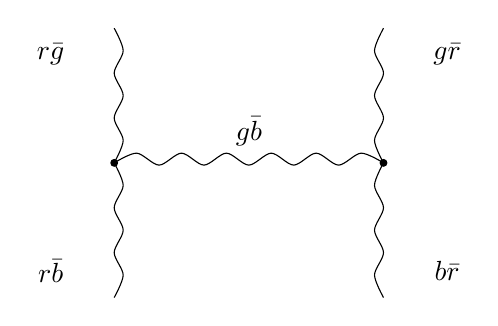
\begin{tikzpicture}[scale=0.95]
\draw[smooth] plot coordinates {
(-1.8,-1.8) (-1.68,-1.50) (-1.80,-1.20) (-1.68,-0.90)
(-1.80,-0.60) (-1.68,-0.30) (-1.8,0)
};
\draw[smooth] plot coordinates {
(-1.8,0) (-1.68,0.30) (-1.80,0.60) (-1.68,0.90)
(-1.80,1.20) (-1.68,1.50) (-1.8,1.8)
};
\draw[smooth] plot coordinates {
(1.8,-1.8) (1.68,-1.50) (1.80,-1.20) (1.68,-0.90)
(1.80,-0.60) (1.68,-0.30) (1.8,0)
};
\draw[smooth] plot coordinates {
(1.8,0) (1.68,0.30) (1.80,0.60) (1.68,0.90)
(1.80,1.20) (1.68,1.50) (1.8,1.8)
};
\draw[smooth] plot coordinates {
(-1.8,0) (-1.50,0.13) (-1.20,-0.03) (-0.90,0.13)
(-0.60,-0.03) (-0.30,0.13) (0,-0.03)
(0.30,0.13) (0.60,-0.03) (0.90,0.13)
(1.20,-0.03) (1.50,0.13) (1.8,0)
};
\node at (-2.65,-1.45) {$r\bar b$};
\node at (-2.65,1.45) {$r\bar g$};
\node at (2.65,-1.45) {$b\bar r$};
\node at (2.65,1.45) {$g\bar r$};
\node at (0,0.42) {$g\bar b$};
\fill (-1.8,0) circle (1.5pt);
\fill (1.8,0) circle (1.5pt);
\end{tikzpicture}
\caption{Austausch eines \(g\bar b\)-Gluons zwischen zwei Gluonen, wobei jede Farb- und Antfarblinie kontinuierlich durch die Vertices verläuft.}
\end{figure}

\section{Gluon-Selbstwechselwirkung und nichtlineare Felder}

Die Gluon-Selbstwechselwirkung verändert den Charakter der QCD. Quarks können durch den Austausch von Gluonen gebunden werden und Hadronen bilden; aber auch Gluonen können durch den Austausch von Gluonen gebunden werden. Die QCD kann daher zusammengesetzte Objekte enthalten, die ausschließlich aus gluonischen Freiheitsgraden bestehen und keine Quarks enthalten. In der QED gibt es kein entsprechendes elementares gebundenes Objekt, das nur aus Photonen besteht.

Die Feldbeschreibung führt zum selben Schluss. Zwei elektromagnetische Wellen durchdringen einander im leeren Raum auf elementarer Ebene, ohne miteinander zu wechselwirken. Zwei Gluonenwellen wechselwirken miteinander und verformen einander. Auch verschiedene Bereiche ein und derselben Gluonenfeldkonfiguration können Kräfte aufeinander ausüben. Das Gluonenfeld ist daher nichtlinear.

\begin{classroomqa}
\audiencequestion{Müssen auf beiden Seiten eines Diagramms gleich viele rote, grüne und blaue Bezeichnungen vorkommen?\lecturetimestamp{01:24:59}}
\lecturerresponse{Die praktische Regel lautet, jeder Farblinie durch das Diagramm zu folgen. Diese Kontinuität ist die Farberhaltung. Kehrt eine Fermionlinie in der Zeit um, wird ihre Bezeichnung zur entsprechenden Antiteilchen- oder Antfarbbezeichnung.}
\end{classroomqa}

\begin{classroomqa}
\audiencequestion{Sind alle Farb- und Antfarbbezeichnungen in der ersten Version des Diagramms konsistent?\lecturetimestamp{01:26:00}}
\lecturerresponse{Nein. Mehrere Bezeichnungen müssen korrigiert werden. Bei einer konsistenten Zuordnung setzen sich die rote, die antblaue und die grüne Linie jeweils durch die Vertices fort; ein umgekehrter Fermionpfeil ist dabei als Antiteilchen zu interpretieren.}
\end{classroomqa}

\begin{classroomqa}
\audiencequestion{Wird eine interne Gluonenlinie als Quark--Antiquark-Paar behandelt?\lecturetimestamp{01:27:58}}
\lecturerresponse{Nur im Sinne der Farbbuchführung. Ein Gluon ist buchstäblich kein zusammengesetztes Quark--Antiquark-Teilchen, trägt aber die entsprechenden Farb- und Antfarbeigenschaften.}
\end{classroomqa}

An diesem Punkt lassen sich die elementaren Regeln knapp zusammenfassen:

\begin{itemize}
\item Quarks emittieren und absorbieren Gluonen;
\item Gluonen wechselwirken direkt mit Gluonen;
\item jede Farb- und Antfarblinie muss kontinuierlich durch einen Vertex verlaufen;
\item wird eine Fermionlinie in der Zeit umgekehrt, geht sie in die entsprechende Antiteilchenlinie über.
\end{itemize}

\begin{classroomqa}
\audiencequestion{Sind Gluonen weiterhin masselos, wenn sie durch all diese Farb--Antfarblinien dargestellt werden?\lecturetimestamp{01:28:13}}
\lecturerresponse{Ja. Gluonen bleiben masselos. Die folgende Einschränkung betrifft die Bedeutung der Masse, die einem Quark im Inneren eines Hadronen zugeschrieben wird.}
\end{classroomqa}

Als Nächstes geht es um das Confinement und den Aufbau der Hadronen: darum, warum isolierte Farbe niemals beobachtet wird und wie sich Quarks und Gluonen im Inneren zusammengesetzter Teilchen organisieren. Zuvor ist es hilfreich, zu klären, was mit der Masse eines Konstituentenquarks gemeint ist.

\section{Sondierungsskala und die Bedeutung der Quarkmasse}

Man stelle sich ein kleines Objekt der Masse \(m\) vor, das an einem weichen, verformbaren Materialstück befestigt ist---ein herunterhängendes Stück Kaugummi genügt als Beispiel. Man übt eine sehr schwache Kraft so langsam aus, dass das weiche Material Zeit hat, sich anzupassen, und sich das ganze System gemeinsam bewegt. Die gemessene Trägheit entspricht dann der Trägheit des kleinen Objekts zusammen mit dem daran befestigten Material.

Nun schüttle man das kleine Objekt mit sehr hoher Frequenz. Das weiche Material hat nicht genug Zeit, der schnellen Bewegung zu folgen. Es bleibt nahezu in Ruhe, während der kleine Kern reagiert. Die gemessene Trägheit bei hoher Frequenz liegt dann viel näher bei \(m\)allein.

\begin{figure}[h]
\centering
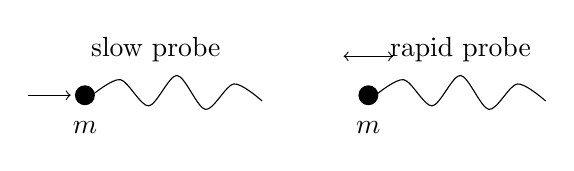
\begin{tikzpicture}[scale=0.9]
\fill (-3,0) circle (4pt);
\node at (-3,-0.45) {$m$};
\draw[smooth] plot coordinates {
(-2.9,0) (-2.5,0.22) (-2.1,-0.15) (-1.7,0.28)
(-1.3,-0.20) (-0.9,0.16) (-0.5,-0.08)
};
\draw[->] (-3.8,0) -- (-3.2,0);
\node at (-2.0,0.65) {slow probe};

\fill (1.0,0) circle (4pt);
\node at (1.0,-0.45) {$m$};
\draw[smooth] plot coordinates {
(1.1,0) (1.5,0.22) (1.9,-0.15) (2.3,0.28)
(2.7,-0.20) (3.1,0.16) (3.5,-0.08)
};
\draw[<->] (0.65,0.55) -- (1.35,0.55);
\node at (2.3,0.65) {rapid probe};
\end{tikzpicture}
\caption{Bei einer langsamen Sondierung bewegen sich der Kern und seine weiche Befestigung gemeinsam; bei einer schnellen Sondierung wird zunächst hauptsächlich die Reaktion des Kerns gemessen.}
\end{figure}

Dies ist eine klassische Analogie. Die erschlossene Masse hängt von der Frequenz der angelegten Kraft ab, weil bei verschiedenen Frequenzen unterschiedliche Teile des Systems Zeit haben, sich an der Bewegung zu beteiligen.

Ein Quark im Inneren eines Hadronen ist von stark wechselwirkendem gluonischem Material und den übrigen Bestandteilen umgeben. Könnte man langsam an einem Quark ziehen, reagierte das ganze Hadron. Die dabei wirksame Trägheit läge dann in der Größenordnung der Nukleonenmasse,
\begin{equation}
m_N\sim930\text{--}940\,\mathrm{MeV}.
\end{equation}
Wird das Quark sehr heftig getroffen und über eine sehr kurze Zeit sondiert, ist die anfängliche Reaktion dem deutlich kleineren Massenparameter zuzuordnen, der einem leichten Quark üblicherweise zugeschrieben wird, ungefähr
\begin{equation}
m_{u,d}\sim5\text{--}10\,\mathrm{MeV}
\end{equation}
bei den hier verwendeten Abschätzungen.

Die Formulierung ``die Masse eines Quarks''erfordert also eine Angabe der Sondierungsskala. Eine sanfte Störung niedriger Frequenz bewegt das ausgedehnte zusammengesetzte Objekt; eine harte Störung hoher Frequenz löst anfänglich nur einen viel kleineren Teil davon auf. Diese Analogie ist keine Herleitung der Renormierung, veranschaulicht aber, warum die zur Beschreibung von Teilchen verwendeten Parameter von den Frequenzen und Wellenlängen der Wechselwirkungen abhängen, bei denen sie gemessen werden. Solche skalenabhängigen Parameter nennt man laufende Parameter oder laufende Konstanten.

\begin{classroomqa}
\audiencequestion{Ist diese frequenzabhängige Masse lediglich eine andere Formulierung einer Unschärferelation wie \(\Delta x\,\Delta t\)?\lecturetimestamp{01:33:32}}
\lecturerresponse{Nein. Das Beispiel beschreibt bereits ein klassisches Phänomen. Eine kleine Masse, die an etwas Weichem befestigt ist, beschleunigt unter einer schnellen Kraft anders als unter einer langsamen, weil unterschiedlich große Teile des befestigten Materials Zeit haben zu reagieren.}
\end{classroomqa}

\begin{classroomqa}
\audiencequestion{Hängt die frühere Diskussion der elektrischen Ladung des Elektrons auf dieselbe Weise von der Skala ab?\lecturetimestamp{01:34:04}}
\lecturerresponse{Ja. Die allgemeine Lehre lautet, dass die zur Beschreibung von Teilchen verwendeten Parameter von den Frequenzen und Wellenlängen der Wechselwirkungen abhängen, bei denen sie sondiert werden. Man nennt sie laufende Konstanten.}
\end{classroomqa}

\begin{classroomqa}
\audiencequestion{Gilt dieselbe Einschränkung für die einem Quark zugeschriebene fraktionale Ladung?\lecturetimestamp{01:34:36}}
\lecturerresponse{Ja. Man muss sorgfältig festlegen, was mit der Ladung eines Quarks gemeint ist. Auf dieser Ebene wird sie relativ zur Protonenladung angegeben; eine vollständigere Definition ist Gegenstand einer gesonderten Diskussion.}
\end{classroomqa}

\editorialnote{Die feste fraktionale elektrische Ladungsquantenzahl und die skalenabhängige Wechselwirkungskopplung sind verschieden. Das Laufen der Kopplung ändert weder die \(+\tfrac23\)- noch die \(-\tfrac13\)-Flavourbezeichnungen selbst.}

\begin{classroomqa}
\audiencequestion{Warum verwendet die Farbbuchhaltung immer ein Quark und ein Antiquark? Warum können nicht zwei Quarks das entsprechende Objekt bilden?\lecturetimestamp{01:34:55}}
\lecturerresponse{Das ist eine wichtige Frage, aber die Antwort gehört in die nächste Diskussion über zulässige Farbkombinationen und Confinement.}\end{classroomqa}

\begin{classroomqa}
\audiencequestion{Wenn einzelne Quarks nicht isoliert werden können, wie hat man dann auf die fraktionale Ladung, die Farbe und das Quarkmodell geschlossen?\lecturetimestamp{01:35:17}}
\lecturerresponse{Das Bild entstand schrittweise aus vielen Hinweisen und scheinbaren Widersprüchen. Regelmäßigkeiten bei Hadronen legten Konstituentenquarks nahe; die Delta-Zustände machten einen Konflikt mit der Fermi-Statistik sichtbar; und das dauerhafte Confinement der Quarks lieferte einen weiteren eigentümlichen Befund. Der Quarkvorschlag entstand in den frühen 1960ern, Nambu entwickelte früh eine wichtige Version der Farbidee, und viele Physiker erarbeiteten und überprüften die vollständige Struktur im Laufe etwa des folgenden Jahrzehnts. Sie ging weder auf eine einzelne Beobachtung noch auf eine einzelne Person zurück.}
\end{classroomqa}

\begin{classroomqa}
\audiencequestion{Warum gibt es nur acht Gluonen statt der scheinbaren neun Kombinationen aus Farbe--und Antfarbe?\lecturetimestamp{01:37:24}}
\lecturerresponse{Die genauere Erklärung dafür, warum die Diagonalsumme kein zusätzliches Gluon darstellt, wird später gegeben.}
\end{classroomqa}

\begin{classroomqa}
\audiencequestion{Werden Elektronen in dieser Diskussion der QCD ausgeklammert?\lecturetimestamp{01:37:33}}
\lecturerresponse{Ja. Die QCD wird hier isoliert betrachtet, so wie man in einer Diskussion der QED vorübergehend Quarks ausklammern kann. Letztlich müssen die getrennten Sektoren zu einer umfassenderen Struktur zusammengeführt werden, die Quarks, Elektronen, Photonen und die übrigen Teilchen enthält. Einige Teile dieser umfassenderen Synthese sind bereits gelungen, andere sind noch unvollständig. In der Physik geht man oft so vor, dass man ein Teilsystem isoliert, es versteht und die Bestandteile anschließend wieder zusammenfügt.}
\end{classroomqa}